\section{Results and Discussion} \label{results}



\subsection{Performance}\label{performance}
\sauliustodo{I think this should be moved somewhere earlier in the report as it justifies the pretext of our work}
The temporal dynamics of a molecular system can be described by the \acrfull{cme}\citationneeded{CME reference}.
\acrfull{gssa}\cite{gillespie_general_1976} simulates these stochastic dynamics directly returning a set of individual trajectories for a list of particles observed.
In order to obtain accurate estimates of the average dynamic within a population of cell (\ie{} the mean dynamics), it is however necessary to perform multiple (often more than $10^4$) simulations.
Despite recent efforts \cite{niemi_efficient_2011,dittamo_optimized_2009,komarov_accelerating_2012} to provide fast implementation of this algorithm, computation remains extremely expensive. \quentintodo{Do you know the Big-Oh complexity?} This time-complexity is a limiting factor in downstream analysis techniques,
for instance parameter inference that often requires repetition of these experiments for a large set of parameter values.

This particular limitation led to the development of approximations such as \acrfull{lna}\cite{komorowski_bayesian_2009} and \acrfull{mea}\cite{ale_general_2013} which model the mean behaviour directly, without evaluating the individual particle behaviours, and therefore can perform in a more realistic time.

Since the main driving force for development of these approximation algorithms is the potential reduction of the time taken to perform the  analysis, it is paramount to make the implementation as efficient as possible.

In this section, we explore the implementation factors that influence the runtime of the algorithm, and describe the optimisations done to increase the performance of it. In particular, we show that symbolic computations can be limiting the algorithm and explain the techniques used to optimised them. We also quantify the increase of performance  and show that it is several order of magnitudes better than the original \mat{} implementation.
In addition, we explore other limiting factors we have less control of, such as the choice of \gls{ode} solver, and discuss their potential implications to the analysis of biological systems.

\subsubsection{Optimising \acrlong{mea}}
\label{sec:optimising_mea}


\gls{mea} involves derivation of a system \gls{ode}s from a model.
This procedure\cite{ale_general_2013}, involves lengthy symbolic calculations.
Even for very simple models (\eg{} three species, five reactions), they cannot be realised manually.
The number equations in the generated \gls{ode} system, for a model with $s$ species and up to moments of order $o$ can be estimated by the following equation: 
\quentintodo[inline]{Does not make sense for 3 species, and 2nd-order moments (3+2-2 choose 3) - 1 = 0}
\begin{displaymath}
    \text{Number of equations} = {{s + o - 2} \choose {s}} - 1
\end{displaymath}
As a consequence, the complexity of the calculation is predicted to increase exponentially with the number of species in the system and the maximal order of moments. \quentintodo[inline]{Add an example numbers illustrating this: "For instance, for a 2-species system ...."}

%In order to perform symbolic computations, we have used \sympy{} \cite{sympy_development_team_sympy:_2014}; a \py{} implementation of
%the symbolic computation routines.

In order to increase the scalability of the method, we have identified significant bottlenecks in our procedures using \py{} profiling tools. We have then attempted to iteratively remove these bottlenecks one by one. Figure~\ref{fig:mea_speed} shows the cumulative effects of different optimisations.

\quentintodo[inline]{Explain why no original python performance line, reduce the detail in caption, make it more evident it is log-normal}


\begin{figure}[tbh]

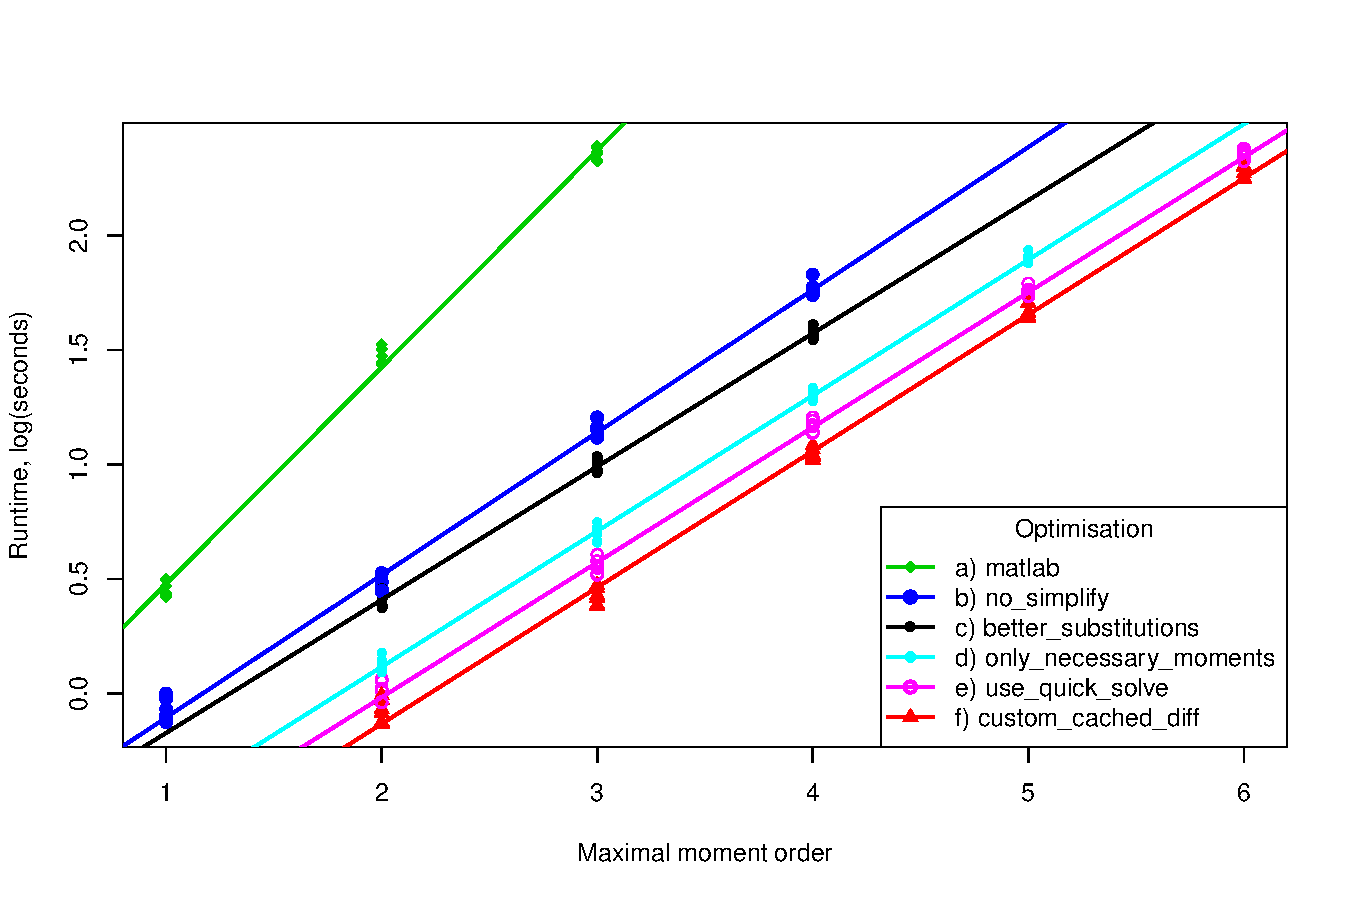
\includegraphics[width=1.0\textwidth{}]{../figure_mea_speed/mea_speed.pdf}
\caption{\emph{Cumulative performance improvement of symbolic calculations resulting from optimisation}.
The processing time for computing log-normal closure on \pft{} model with different maximal moment orders were measured for original Matlab implementation (a) and different optimisations (b$-$f).
In a first place, the calls to \texttt{sympy.simplify()} where removed (b). 
Then, \texttt{sympy.xreplace()} was used instead of \texttt{sympy.substitute()} (c). 
Generating an $(n-s) \times (n_2-s + 1)$ matrix (d), as opposed to an $(n-s) \times (n-s + 1)$ one, also increase speed (see main text).
Implementing a simplified equation solver instead of using \texttt{sympy.solve()} also resulted in a significant speed-up (e). Finally, caching (memorisation) \texttt{sympy.diff()} allowed even better performance.
The time complexity appears exponential ($O(2^n)$, where $n$ is the maximal moments order) in every case, 
Interestingly, the slopes between, a ($0.95$) and c ($0.58$), and b ($0.62$) and c were significantly different ($p-value <10^{-15}$ and $p-value = 3 \times 10^{-4}$, respectively; t-test on the slopes of the linear regression). 
No significant difference was found between the slopes of the subsequent optimisations (c$-$f). 
However, the intercepts were significantly smaller between each consecutive optimisations after c) ($p-value < 10^{-6}$ for all; t-test on the intercepts of the linear regression).
Nine replicates were performed on the same CPU. For optimisation c$-$f, values corresponding to maximal order moments lower than two were removed because of the inherent inaccuracy in measuring very short durations}
\label{fig:mea_speed}
\end{figure}

\quentintodo[inline]{Simplify this, move out the specific details to your individual report, it is enough to give just the overview here.}

The first step involved removing the expression simplification heuristic.
In the original code\footnote{both from the publication and last year's MSc project}, the right-hand-side equations were simplified in order to produce shorter text file results.
However, this was slow and did not benefit subsequent simulations and inference.
For large expressions, simplification had also had an large memory footprint and was likely to fail.
This optimisation significantly improved the scalability of the method (see fig.~\ref{fig:mea_speed}, b).

The next bottleneck was the choice of substitution functions.
As a part of \gls{mea}, it is necessary to replace raw moment symbols by expressions depending on central moments.
Performing substitution can be done using the \texttt{substitute()} function from \sympy, but this is designed to substitute expressions by other expressions.
In most cases, we only had to substitute atomic symbols by expression.
For this purpose, the  \texttt{xreplace()} function was a much more appropriate alternative which resulted in a better scalability (see fig.~\ref{fig:mea_speed}, c).

In the original implementation, a matrix of central moment expression of size $(n-s) \times (n-s + 1)$ is directly generated when the default closure is applied.
However, when using a parametric closure, a matrix of size $(n_2-s) \times (n_2-s + 1)$, where $n_2={{s+o-2 \mathbf{+1}} \choose {s}} -1$, was generated.
The $n_2 - n$ rows corresponding to higher-order moments have then to be deleted.
In contrast, out implementation generates a $(n-s) \times (n_2-s + 1)$ matrix regardless of the closure method.
In addition to improve code readability, consistency and flexibility \footnote{see QG's individual report}, this improved overall performance (fig.~\ref{fig:mea_speed}, d) for cases where closure is applied while keeping the default closure computation fast.

Another simple way to improve computation time was to remove calls to the function \texttt{solve()} which was only used in straightforward cases (\eg{} solving: $a + 2b = c$ for $a$).
It was therefore much more efficient (fig.~\ref{fig:mea_speed}, e) to use simple arithmetic to find solution.

Finally, partial derivation of expression over several variables and order is extensively performed during the approximation.
Generally, these type of differentiations can be simplified several differentiation of first order:
\begin{equation}
\frac{\partial{} ^ 2 f(x,y)}{\partial x \partial y}  =
\frac{\partial{} \frac{\partial{} f(x,y)}{\partial x}}{\partial y} =
\frac{\partial{} \frac{\partial{} f(x,y)}{\partial{} y}}{\partial{} x}
\end{equation}
One advantage, is that, when needing to calculate two derivatives such as:  $\frac{\partial{} ^ 2 f(x,y)}{\partial{} x \partial{} y}$ and $\frac{\partial{} ^ 2 f(x,y)}{\partial{} x^2}$, 
one can precompute $\frac{\partial{} f(x,y)}{\partial{} x}$ and use it for both calculation.
In our implementation, we have use a procedure known as \emph{memorisation} which, briefly, permits to store the results of a function call in an associative array.
Then, the next time this function is called with the same arguments, it will return the stored results instead of recomputing it.
This also resulted in an overall performance improvement (fig.~\ref{fig:mea_speed}, f).

In conclusion, reorganising, profiling and rewriting the code resulted in incremental significant performance improvements of symbolic computations in \means{} compared to the original \mat{} code.
For instance, with the same \pft{} system and closure method, 
we predict that computation up to \gls{ode}s up $8^{th}$ order will take 44 minutes with \means{} and as much as 128 days with the original implementation.\quentintodo{Add a number saying how long it would have taken for the first iteration of optimisation as well.}
These improvement have allowed us to explore the performance of MEA in higher depth, and will hopefully contribute to make \gls{mea} realistically usable for systems with more species and reactions.

\subsection{Moment Expansion Closure}

In \gls{mea} the temporal derivative of each central moment is expressed in terms of the higher order moment. 
This behaviour essentially has no upper bound and continues to the moments of infinite order. 
Since we cannot evaluate these expressions in the limit analytically, it is necessary to ``close'' the expansion by providing a closed form for the higher order moments. This also makes the method an ``aproximation" rather than an exact method.

In the original work \cite{ale_general_2013}, higher order central moments are assumed to be equal to zero. This is very clean mathematically, but is a strong and not necessarily valid assumption. 

As an alternative, parametric probability distribution can be used to express moments of arbitrary orders. 
For instance, a multivariate normal distribution is parametrised only by means (\ie{} first order raw moment)
and a covariance matrix (\ie{} second order central moments). 
As a consequence, it is possible to express any arbitrary moment from means, variances and covariances. 
A promising area of research involves closing moment expression by parametric forms of highest order central moments instead
of assuming them to be null.
Preliminary work \citationneeded{Eszter, unpublished} suggests that using a parametric distributions for \gls{mea} \quentintodo[inline]{Finish this sentence!}
In addition, Ale \emph{et al.} predicted that higher maximal moment order would \quentintodo{are you sure? didn't Michael deny this}necessarily result in better approximation \cite{ale_general_2013}.

The dramatic improvement in performance compared to the \mat{} prototype (see \autoref{sec:optimising_mea}) has made it possible for us to explore the dynamics of both the higher-order and probabilistic moment closures and verify the claims about their performance efficiently.

\quentintodo[inline]{Consider making this figure a barchart}
\begin{figure}[t]
    \centering
    \includegraphics[width=1.0\textwidth]{../pipeline/task-output/FigureP53Summary/FigureP53Summary-pdf-7.pdf}
    \caption{\emph{Effect of different closure methods and maximal moment order on simulation accuracy}. The \pft system was modelled using \gls{mea} with five types of closure and for maximal moment order up to seven.
Resulting trajectories were all compared to an average of 5000 \gls{gssa} simulations using sum of square distance (a).
Distance is in log scale. Missing values indicate solver failure for that particular set of parameters.}
    \label{fig:max_order_and_closure_on_distance_summary}
\end{figure}


Figure~\ref{fig:max_order_and_closure_on_distance_summary} summarises the effect of increasing maximal moment order and different type of closures.
The \pft{} system, with parameters from \cite{ale_general_2013}, was investigated.
As mentioned earlier it is expected that the approximation accuracy increases as the maximal moment order does, \ie{} distance to \gls{gssa} obtained means decreases as maximal moment order increases. 
This trend is true for for normal and scalar closures, up to maximal moment order six. 

This trend is not true for the seventh order moment, though.
\quentintodo[inline]{Todo double check the labels in the legend, was it really normal that was worse and scalar that failed?}
As seen in the figure, the closure using the normal distribution had performed worse than the sixth order closure when maximum order was set to seven.
We could not obtain the result for the seventh order closure using the standard scalar closure, as the ODE solver has failed simulating the problem, which usually indicates a stiff \gls{ode} problem. 
The generated trajectories are shown in the \autoref{fig:max_order_and_closure_on_distance_trajectories}. One can see the trajectory generated from the normal distribution closure mismatch the trajectory obtained from the \gls{gssa} simulations by quite a wide margin (\emph{purple line, subplot on the right-hand-side}). 

It is hard to determine the reason for this behaviour, it might be a limitation of the approximation method, or a limitation of the \gls{ode} solver available. It is hard to know which explanation is more likely as, we cannot test the two hypotheses separately. All we can say is that have been able to observe a similar behaviour with all of the solvers tested, which is further explored in \sauliustodo{link to my section where we study the phenomenon on larger scale with different solvers}.

\quentintodo{I cannot see that to be true, from the figure}
Note that for even maximal moment orders, normal and scalar are rigorously equal.
\quentintodo{Not intuitive to me, explain}This is expected since normal distribution is symmetrical (\emph{i.e.} odd central moments are always zero).

\begin{figure}
    \centering
    \includegraphics[width=1.0\textwidth]{../pipeline/task-output/FigureP53Simple/FigureP53Simple-pdf-7.pdf}
%~
    \caption{\emph{Complete trajectories of a single species (\pft) for max order three and seven are shown} Black lines indicate the average of \gls{gssa} simulations. Missing lines, compared to the legend in \autoref{fig:max_order_and_closure_on_distance_summary} indicate solver failure.}
    \label{fig:max_order_and_closure_on_distance_trajectories}
\end{figure}

Log-normal closure method is also displaying a similar behaviour with regards to the approximation of ground truth trajectories, though less extreme. 
The ground truth trajectory seems to be well approximated when the maximal moment order is three, but the approximation gets less and less accurate for higher maximal order moments.
A deeper look at the trajectories indicate that, in this latter case,
oscillations are damped too quickly, as opposed to the behaviour seen using normal closure, where the oscillation amplitude increases (see \autoref{fig:max_order_and_closure_on_distance_trajectories}, red line).

\quentintodo{what?} Interestingly for even maximum moment order log-normal closures generated \gls{ode}s which,
despite our efforts, could not be numerically solved.

Finally, it seems that the results obtained from multivariate distribution closures and  univariate distribution closures, which do not model the covariance terms, are the same for this particular system. 
This is not true for all of the systems. For instance, we have observed that in the \emph{hes1}, it is advantageous to model covariance (data not show\quentintodo{show data, otherwise our point is weak}).

The results in this section show that, while it might be convenient to believe that using higher order moments would provide better approximations, the results indicate that this is not necessarily the case as there seems to be the \emph{sweet spot} parameter set that gives the best results. Unfortunately, this makes it difficult to \emph{a priori} define which closure and maximal moment order should be used for a given system. The section \sauliustodo{link to the section} explores this phenomenon on wider scale of parameters.

\subsection{Parameter Inference using \acrlong{mea}}
Parameter inference procedure aims to obtain the correct parameter values for the system by exploring the parameter space and comparing the simulation trajectories with the experimental data. 

In order to study the performance of the parameter inference procedure using \acrlong{mea}, we took the average trajectory obtained from the  $5000$ \gls{gssa} simulations of the \pft{} with a certain parameter set and used it as the observed dataset we want to infer the parameters from. Essentially, the inference procedure is expected to return the said parameter set back to us.

In order to determine the base case performance, we performed the parameter inference using the \pft{} model expressed only in terms of the first order moments. This approximation is bound to be very inaccurate for the particular system, as higher order moments are necessary to capture the damped oscillations present in the means of \gls{gssa} simulations\cite{ale_general_2013}\sisitodo{figure is needed}.

We have started parameter inference procedure at the correct parameter values, expecting to see an immediate result and no movement in the parameter space. To much of our surprise, however, when the inference is allowed to navigate the complete parameter space, not only did the procedure move around, but it was able to find a set of parameters, that when expressed in terms of first order moments, are able to match the observed trajectories completely.

The set of parameters obtained by the inference were very different from the actual SSA simulations, but the approximated trajectories were identical. This strongly questions the suitability of parameter inference procedures in obtaining the correct parameter sets.

\sisitodo[inline]{Need figure here showing that they are really close}
\sisitodo[inline]{Why don't we compare the SSA trajectories with these parameters somewhere as well, if there is time?}

In order to gain some insight into the reason of unexpected inference performance, we first attempted to restrict ourselves to easier to comprehend two-dimensional space.
To do this, we restricted our parameter inference procedure to only move through pair of parameters only, while all other parameters are fixed (to their true values). 
We performed this for all combinations of two parameters and checked if we can reproduce the curious behaviour.

Interestingly, we were able to observe the same behaviour for the parameter pairs $c_0$ and $c_6$, $c_1$ and $c_2$, and finally $c_2$ and $c_6$.
\begin{figure}
\includegraphics[width=0.95\textwidth]{../pipeline}
\caption{\emph{Parameter pair $c_2$ and $c_6$ can produce a perfect match between inferred optimal trajectories and SSA trajectories for all species in \pft{} model.}}
\label{fig:}
\end{figure}

We have chosen the pair of parameters that allowed the inference procedure to converge to a trajectory with minimal distance to the stochastic average -- $c_2$ and $c_6$ for further investigations.
 
\sisitodo[inline]{See the commented text below this todo -- instead of it please talk a bit more about how the landscape looks for the max\_order = 1. Then go on and talk about higher-order moments, explicitly mentioning that you were able to find close-enough trajectories for all of them, however, neither of them were accurate parameter wise}
%If the inference method was correct, the starting point in the distance landscape would already have a low distance, and the end point should overlap with the starting point, i.e. the true values of $c_2$ and $c_6$.

In conclusion, the data makes us question the validity of parameter inference approaches using \gls{mea} approximation.
As seen in \sisitodo{remind which figures} distance landscape shows that the starting point (which is the correct parameter set) can be distant from the minima. Similarly, the distance procedure, if uncontrolled, is able to find itself exploring the values for some parameters (i.e. $c_6$) that are more than 10 times larger than the true value, which not be very meaningful biologically.\sisitodo{great point, but also needs coverage above}
\sisitodo{not clear what you meant here}Finally, the trajectories for all the species in the p53 model sometime demonstrate misfit between the optimal trajectory obtained from inference and the "observed trajectory" from \gls{gssa}. 

\sisitodo[inline]{I think you should structure your figures as you did initially -> the landscape on the left, trajectories on the right, and have one figure per combination of the two}

\begin{figure}
\centering
    \begin{subfigure}[t]{0.2\textwidth}
    \includegraphics[width=\textwidth]{{../pipeline/task-output/SampleMultidimensionInferenceFigure/SampleMultidimensionInferenceFigure-pdf-1-scalar-True-90.0_0.002_1.704_1.1_0.93_0.96_0.7822-ode15s--90.0_0.002_1.704_1.1_0.93_0.96_0.7822-sum_of_squares-5000}.pdf}
    \end{subfigure}
    \begin{subfigure}[t]{0.2\textwidth}
    \includegraphics[width=\textwidth]{{../pipeline/task-output/SampleMultidimensionInferenceFigure/SampleMultidimensionInferenceFigure-pdf-2-scalar-True-90.0_0.002_1.704_1.1_0.93_0.96_0.7822-ode15s--90.0_0.002_1.704_1.1_0.93_0.96_0.7822-sum_of_squares-5000}.pdf}
    \end{subfigure}
    \begin{subfigure}[b]{0.2\textwidth}
    \includegraphics[width=\textwidth]{{../pipeline/task-output/SampleMultidimensionInferenceFigure/SampleMultidimensionInferenceFigure-pdf-3-scalar-True-90.0_0.002_1.704_1.1_0.93_0.96_0.7822-ode15s--90.0_0.002_1.704_1.1_0.93_0.96_0.7822-sum_of_squares-5000}.pdf}
    \end{subfigure}
    \begin{subfigure}[b]{0.2\textwidth}
    \includegraphics[width=\textwidth]{{../pipeline/task-output/SampleMultidimensionInferenceFigure/SampleMultidimensionInferenceFigure-pdf-4-scalar-True-90.0_0.002_1.704_1.1_0.93_0.96_0.7822-ode15s--90.0_0.002_1.704_1.1_0.93_0.96_0.7822-sum_of_squares-5000}.pdf}
    \end{subfigure}
    \begin{subfigure}[b]{0.2\textwidth}
    \includegraphics[width=\textwidth]{{../pipeline/task-output/SampleMultidimensionInferenceFigure/SampleMultidimensionInferenceFigure-pdf-5-scalar-True-90.0_0.002_1.704_1.1_0.93_0.96_0.7822-ode15s--90.0_0.002_1.704_1.1_0.93_0.96_0.7822-sum_of_squares-5000}.pdf}
    \end{subfigure}
    
\caption{\emph{Distance landscape at different maximal orders for p53 model.} In the landscape, the warmer the colour, the more distant the inferred trajectories are from the \gls{gssa} trajectories. 
The \gls{gssa} trajectories are generated using the new parameter values labelled as \emph{start}. Among seven parameters, only the values for $c_2$ and $c_6$ are inferred, with starting values inferred from inference using the true values.} 
\label{fig:parameter_inference_landscape}
\end{figure}

\begin{figure}
\centering
    \begin{subfigure}[b]{0.6\textwidth}
    \includegraphics[width=\textwidth]{{../pipeline/task-output/FigureInferenceStartEndSSA/FigureInferenceStartEndSSA-1-scalar-c2-1.7040-c6-0.7822}.pdf}
    \end{subfigure}
    \begin{subfigure}[b]{0.6\textwidth}
    \includegraphics[width=\textwidth]{{../pipeline/task-output/FigureInferenceStartEndSSA/FigureInferenceStartEndSSA-2-scalar-c2-1.7040-c6-0.7822}.pdf}
    \end{subfigure}
    \begin{subfigure}[b]{0.6\textwidth}
    \includegraphics[width=\textwidth]{{../pipeline/task-output/FigureInferenceStartEndSSA/FigureInferenceStartEndSSA-3-scalar-c2-1.7040-c6-0.7822}.pdf}
    \end{subfigure}
    \begin{subfigure}[b]{0.6\textwidth}
    \includegraphics[width=\textwidth]{{../pipeline/task-output/FigureInferenceStartEndSSA/FigureInferenceStartEndSSA-4-scalar-c2-1.7040-c6-0.7822}.pdf}
    \end{subfigure}
    \begin{subfigure}[b]{0.6\textwidth}
    \includegraphics[width=\textwidth]{{../pipeline/task-output/FigureInferenceStartEndSSA/FigureInferenceStartEndSSA-5-scalar-c2-1.7040-c6-0.7822}.pdf}
    \end{subfigure}
\caption{\emph{Trajectories for each species in p53 model using different maximal orders.} 
Three trajectories are shown for each species. 
The starting trajectories are simulated using the starting values are indicated above the trajectories, with $c_2$ and $c_6$ inferred using \emph{sum of squares} distance method. 
Both the optimal and the \gls{gssa} trajectories are generated based on the end point in correspondent distance landscape in Figure 5.} 
\label{fig:parameter_inference_trajectories}
\end{figure}
